\documentclass[border=4pt]{standalone}
\usepackage[utf8]{inputenc}
\usepackage[T1]{fontenc}
\usepackage{amsmath,amssymb}
\usepackage[table]{xcolor}
\usepackage{tikz}
\usetikzlibrary{positioning,fit,calc,arrows.meta,shapes.geometric,decorations.pathreplacing,backgrounds}
\usepackage{pgfplots}
\pgfplotsset{compat=1.17}
\definecolor{stellantis}{RGB}{26,58,92}
\definecolor{sectionblue}{RGB}{44,95,138}
\definecolor{ddbrown}{RGB}{180,100,30}
\definecolor{ddbrownlight}{RGB}{255,243,230}
\begin{document}

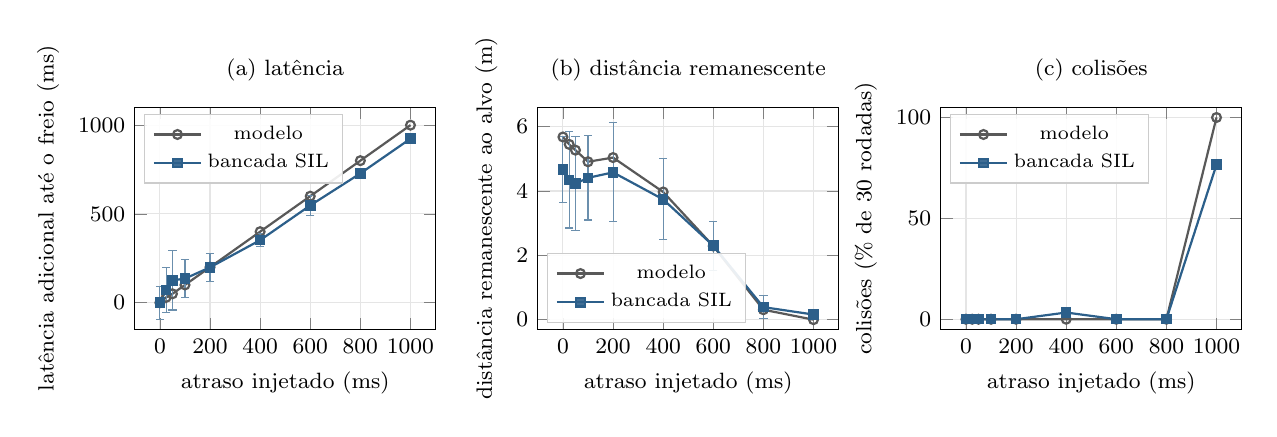
\begin{tikzpicture}
\begin{axis}[/pgf/number format/use comma, /pgf/number format/1000 sep={}, width=5.4cm, height=4.4cm, grid=major, grid style={gray!20}, tick label style={font=\footnotesize},
label style={font=\footnotesize}, legend style={font=\scriptsize, draw=gray!40, fill=white, fill opacity=0.9, text opacity=1},
xlabel={atraso injetado (ms)}, xtick={0,200,400,600,800,1000}, name=a, ylabel={latência adicional até o freio (ms)}, ymin=-150, ymax=1100,
  legend pos=north west, title={\footnotesize (a) latência}]
\addplot[gray!50, dotted, domain=0:1000, forget plot] {x};
\addplot[color=gray!70!black, mark=o, mark size=1.6pt, thick] coordinates {(0,0.00) (25,30.00) (50,50.00) (100,100.00) (200,200.00) (400,400.00) (600,600.00) (800,800.00) (1000,1000.00)}; \addlegendentry{modelo}
\addplot[color=sectionblue, mark=square*, mark size=1.5pt, thick, error bars/.cd, y dir=both, y explicit, error bar style={sectionblue!70}] coordinates {(0,0.00) +- (0,93.59) (25,70.68) +- (0,127.41) (50,125.24) +- (0,166.52) (100,135.88) +- (0,106.72) (200,199.15) +- (0,77.38) (400,352.11) +- (0,34.97) (600,547.88) +- (0,55.90) (800,728.19) +- (0,15.36) (1000,923.75) +- (0,14.32)}; \addlegendentry{bancada SIL}
\end{axis}
\begin{axis}[/pgf/number format/use comma, /pgf/number format/1000 sep={}, width=5.4cm, height=4.4cm, grid=major, grid style={gray!20}, tick label style={font=\footnotesize},
label style={font=\footnotesize}, legend style={font=\scriptsize, draw=gray!40, fill=white, fill opacity=0.9, text opacity=1},
xlabel={atraso injetado (ms)}, xtick={0,200,400,600,800,1000}, at={(a.east)}, anchor=west, xshift=1.3cm, name=b, ylabel={distância remanescente ao alvo (m)},
  ymin=-0.3, ymax=6.6, legend pos=south west, title={\footnotesize (b) distância remanescente}]
\addplot[color=gray!70!black, mark=o, mark size=1.6pt, thick] coordinates {(0,5.68) (25,5.45) (50,5.27) (100,4.91) (200,5.04) (400,3.97) (600,2.29) (800,0.31) (1000,0.00)}; \addlegendentry{modelo}
\addplot[color=sectionblue, mark=square*, mark size=1.5pt, thick, error bars/.cd, y dir=both, y explicit, error bar style={sectionblue!70}] coordinates {(0,4.67) +- (0,1.02) (25,4.35) +- (0,1.50) (50,4.23) +- (0,1.47) (100,4.41) +- (0,1.31) (200,4.58) +- (0,1.54) (400,3.74) +- (0,1.26) (600,2.30) +- (0,0.76) (800,0.39) +- (0,0.36) (1000,0.16) +- (0,0.08)}; \addlegendentry{bancada SIL}
\end{axis}
\begin{axis}[/pgf/number format/use comma, /pgf/number format/1000 sep={}, width=5.4cm, height=4.4cm, grid=major, grid style={gray!20}, tick label style={font=\footnotesize},
label style={font=\footnotesize}, legend style={font=\scriptsize, draw=gray!40, fill=white, fill opacity=0.9, text opacity=1},
xlabel={atraso injetado (ms)}, xtick={0,200,400,600,800,1000}, at={(b.east)}, anchor=west, xshift=1.3cm, ylabel={colisões (\% de 30 rodadas)},
  ymin=-5, ymax=105, legend pos=north west, title={\footnotesize (c) colisões}]
\addplot[color=gray!70!black, mark=o, mark size=1.6pt, thick] coordinates {(0,0.00) (25,0.00) (50,0.00) (100,0.00) (200,0.00) (400,0.00) (600,0.00) (800,0.00) (1000,100.00)}; \addlegendentry{modelo}
\addplot[color=sectionblue, mark=square*, mark size=1.5pt, thick] coordinates {(0,0.00) (25,0.00) (50,0.00) (100,0.00) (200,0.00) (400,3.33) (600,0.00) (800,0.00) (1000,76.67)}; \addlegendentry{bancada SIL}
\end{axis}
\end{tikzpicture}
\end{document}
